\documentclass[./main.tex]{subfiles}

\begin{document}

%%----------------------------------------------------
\begin{figure}[H]
\centering
\includegraphics[width=\textwidth]{resources/sequence_diagrams/safeReports1}
\caption{First part of SafeReport}
\end{figure}

The user takes a picture using the mobile app. The needed metadata
(GPS coordinates, timestamp) are then automatically captured by the app.
The user needs to select the type of violation from a predefined list.
After selecting the violation type the violation report is generated and
forwarded to the router. The router must determine the right component for the new violation report. The report is sent to the report manager a SafeReports subcomponent that can handle all the new requests for violation reports.
The report manager wants to retrieve the license plate of the violation
and to achieve that goal, it sends the picture contained in the
violation report to the picture manager.
The picture manager forwards the picture to the external OCR software.
If the OCR is not able to read the license plate then an error message is
sent in a cascade mode back to the user, who is asked to repeat the entire process. The process ends.
\\Otherwise, the license plate is returned to the picture manager and then to the report manager.
Once the report manager has the license plate it sends the completed report to the DBMS. The violation report is temporarily stored in the database. After that, the DBMS sends an acknowledge to the report manager. Then the report manager sends the license plate to the router and from it to the app.
\\It is important to notice that the violation reports temporarily stored are deleted after a small fixed amount of time. When a violation report temporarily stored is automatically deleted it means that the user never confirmed the license plate of that violation report. This situation is better explained in the second part of the SafeReports sequence diagram.

%%-----------------------------------------------------
\begin{figure}[H]
\centering
\includegraphics[width=\textwidth]{resources/sequence_diagrams/safeReports2}
\caption{Second part of SafeReports}
\end{figure}

The user needs to confirm or refuse the license plate.
If the user doesn't confirm the plate then a \textit{user denial} is sent to the report manager passing through the router. The report manager sends a request to the DBMS to delete the temporary violation report if any. The DBMS sends the acknowledge of the deletion to the report manager. The report manager sends the reply to the router and from it to the app. The process ends.\\
Otherwise, a \textit{user confirmation} is sent to the router and then to the report manager.
The report manager wants to store the new violation report and to do that it forwards the report to the DBMS. The DBMS tries to retrieve the corresponding violation report from the temporary data. After retrieving the temporary report the DBMS checks if there is no other equivalent violation report already permanently stored in the database.
If something goes wrong during the retrieval or if the DBMS finds an equivalent report already permanently stored into the database then it doesn't update the database and it sends an error to the report manager. An error is sent to the user passing through the router and the mobile app. The process ends.\\
Otherwise, the DBMS is able to permanently store the new violation report in the database and then a positive reply is sent to the report manager. The report manager sends a positive reply to the router and then to the mobile app. The user is notified about the successful operation. The process ends.\\
We tried to emphasize the differences between storing violation reports temporarily or permanently. Temporary reports are reports that are waiting for a confirmation from the user. Permanent reports are reports that have already the user confirmation and are stored in the database forever.\\
We need to notice that every time the report manager is notified that a new violation report is permanently stored in the DBMS then the \textit{generate tickets} process starts in parallel.


%%-----------------------------------------------------

\begin{figure}[H]
\centering
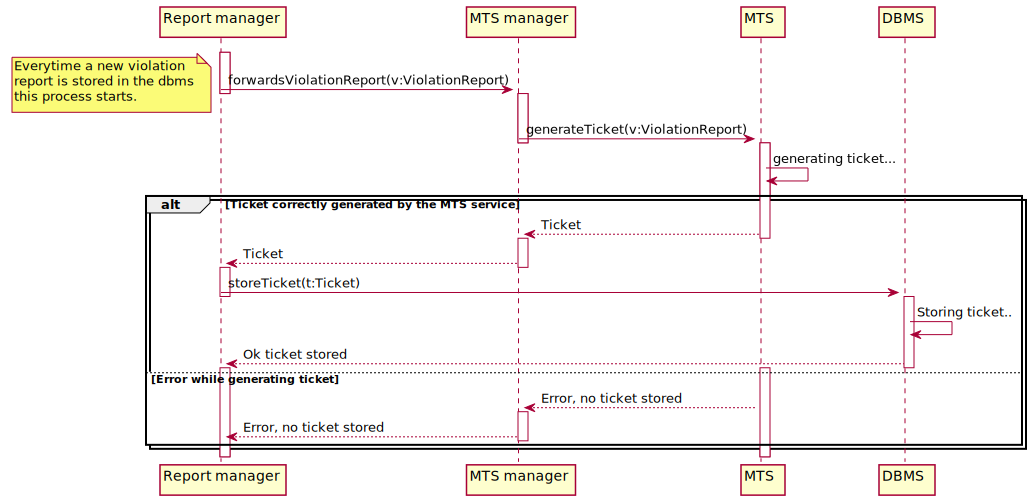
\includegraphics[width=\textwidth]{resources/sequence_diagrams/generate_tickets}
\caption{Generate tickets from reports}
\end{figure}

Every time a new violation report is permanently stored in the database this process starts.
The report manager sends the stored violation report to the MTS
manager. This process is done in parallel with the SafeReports process.
Since MTS manager wants to generate a ticket it forwards the violation
report to the MTS.
If the MTS is not able to generate the ticket then it forwards an error to the MTS manager. The MTS manager propagates the error to the report manager and the process ends.\\
Otherwise, the generated ticket is sent to the MTS manager and then to the report manager. It forwards the new ticket to the DBMS to store the ticket.
After the ticket is stored in the database the DBMS sends a confirmation to the report manager and the process ends.

%%-----------------------------------------------------
\begin{figure}[H]
\centering
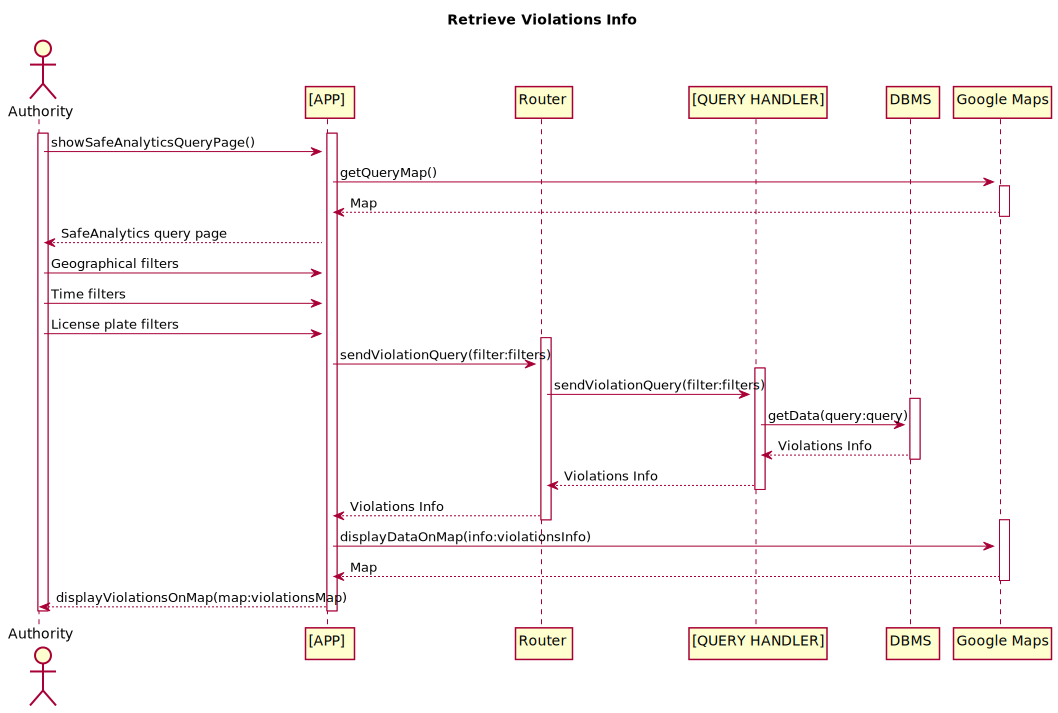
\includegraphics[width=\textwidth]{resources/sequence_diagrams/retrieve_violation_info}
\caption{Get information about reported violations}
\end{figure}

Here is shown how authorities get access to the information about the reported violations. This diagram is very similar to the one for the same functionality for the common user, so instead of representing it twice, the differences will be highlighted in this description.\\
The user is shown the SafeAnalytics main page, which consists in a query interface, changing according to the type of user. While common users are asked to insert position and time ranges, authorities can also ask for specific license plates. The selection of the position filter requires to display a map, so Google Maps is involved.\\
All the query data provided are stored in a Filter object and the query is passed to the DBMS, to retrieve the required data from the DB. This does not happen in a single step, as the request must pass through the Router and the QueryHandler. The response is sent back to UserApplication, which displays it on a map thanks again to Gooogle Maps.


%%-----------------------------------------------------
\begin{figure}[H]
\centering
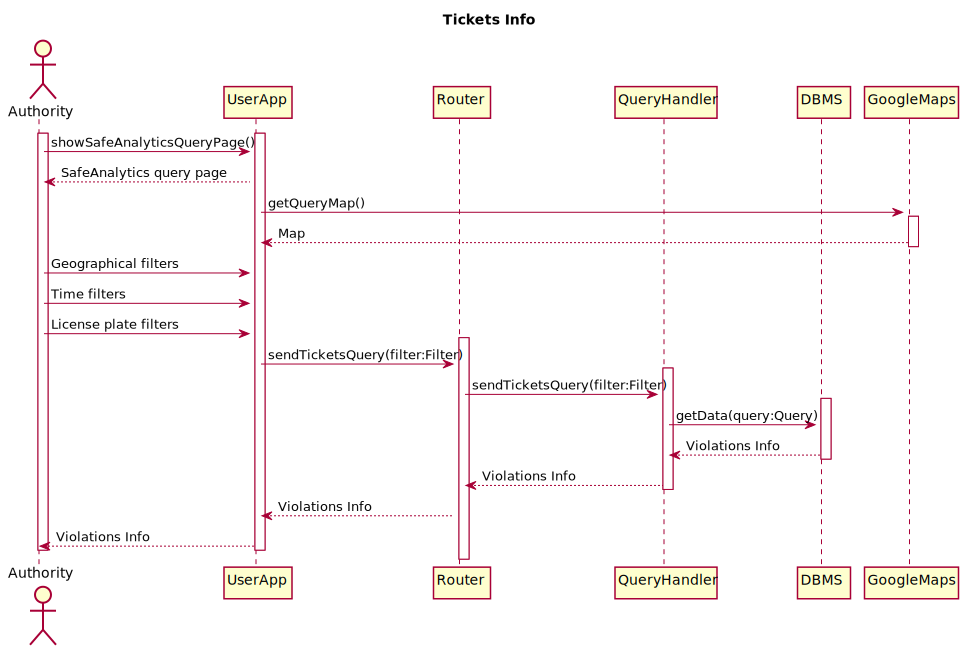
\includegraphics[width=\textwidth]{resources/sequence_diagrams/tickets_info}
\caption{Get information about generated tickets}
\end{figure}

Authorities get an interface similar to the one for getting information about the violations to get the tickets data. In the same way as for the other authority queries, a request for the information is forwarded to the DBMS. The statistics are not shown in a map (so Google Maps is not involved anymore), and the data flows back on the same path of the request to the user.

%%-----------------------------------------------------
\begin{figure}[H]
\centering
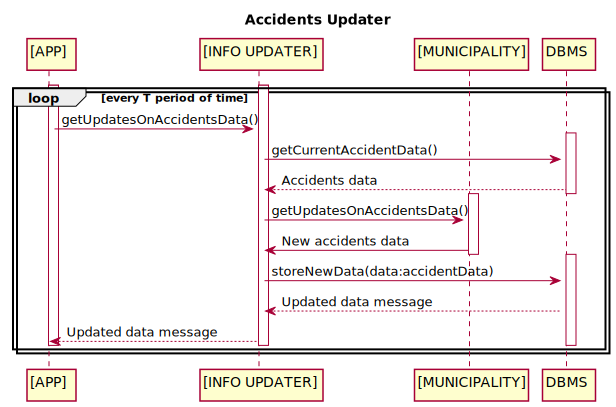
\includegraphics[width=\textwidth]{resources/sequence_diagrams/info_updater}
\caption{Update data from municipality}
\end{figure}

The system must periodically collect the accidents' data provided by the municipality. To do so, InfoUpdater contains a trigger to ask for new data. In order to not download the whole dataset provided by the municipality every time, a time stamp is saved to get the latest data only.

%%-----------------------------------------------------

\begin{figure}[H]
\centering
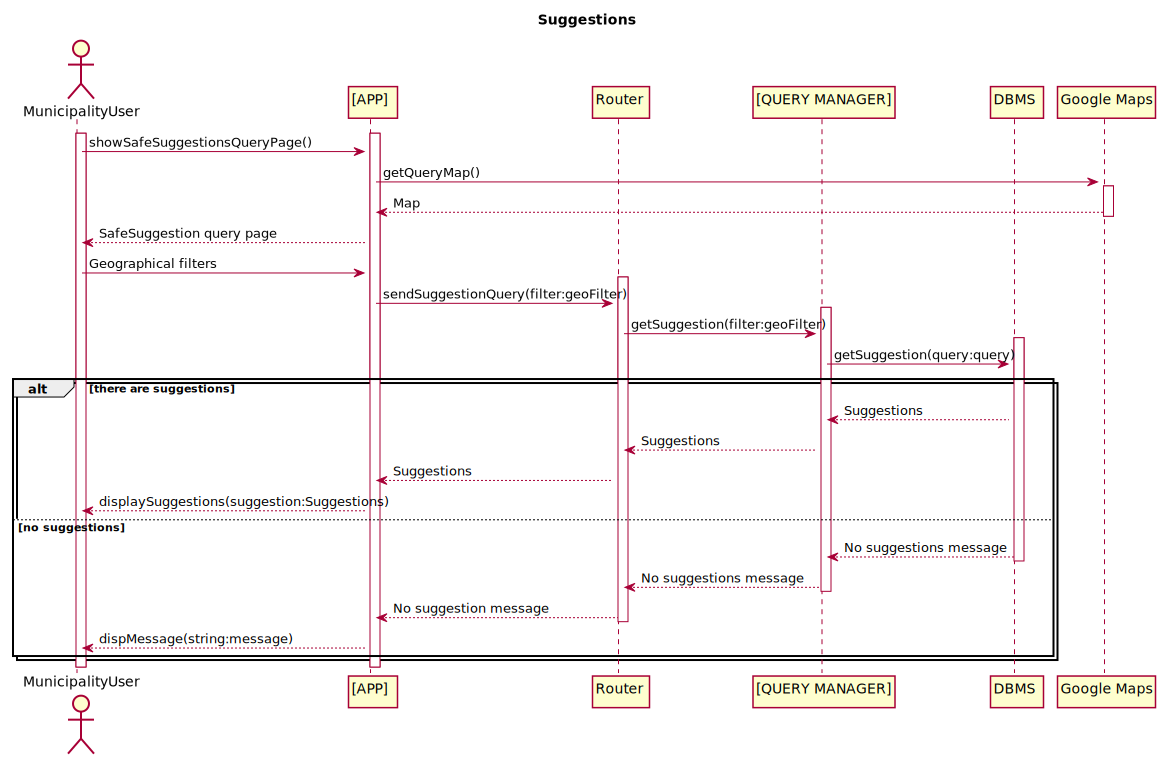
\includegraphics[width=\textwidth]{resources/sequence_diagrams/suggestions}
\caption{Get suggestions}
\end{figure}

%TODO maybe the data warehouse should be shown

The municipality user can get suggestions from a query page similar to the ones provided to the other users, but where the filters are only geographical. The DBMS gives an answer, which can be negative or a suggestion.

\end{document}
